\section{E-Mail}
\begin{frame}{E-Mails: Was soll geschützt werden?}
  E-Mails können
  \begin{itemize}
    \item abgehört
    \item gefälscht
  \end{itemize}
  werden. Deshalb stellen wir vor, wie man
  \begin{itemize}
    \item die Vertraulichkeit (das ,,Briefgeheimnis``) umsetzt
    \\ $\Rightarrow$ Verschlüsselung
    \item die Echtheit des Gegenübers sicherstellt
    \\ $\Rightarrow$ Digitale Signatur
  \end{itemize}
  Außerdem:
  \begin{itemize}
    \item Wie man sicherstellt, dass sein E-Mail Passwort\\ nicht einfach mitgelesen werden kann
  \end{itemize}
\end{frame}

\begin{frame}{E-Mail}{Funktionsweise}
  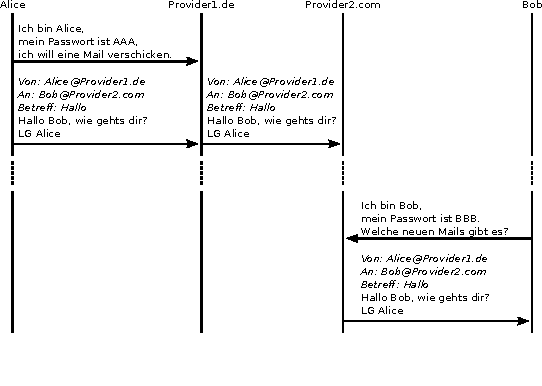
\includegraphics[width=.9\textwidth]{images/maildaten.pdf}
  \scriptsize
  ~\\
  ~\\
\end{frame}

\begin{frame}{E-Mail}{Transportverschlüsselung (SSL/TLS bzw. STARTTLS)}
  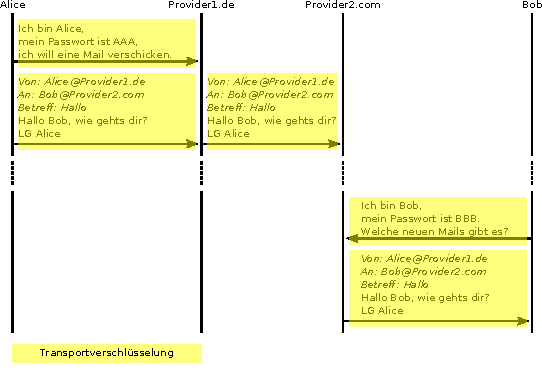
\includegraphics[width=.9\textwidth]{images/maildaten_trans.pdf}
  \begin{itemize}
    \scriptsize
    \item muss von den Mailanbietern unterstützt werden
    \item Konfiguration des Mailprogramms überprüfen!
  \end{itemize}
\end{frame}

\begin{frame}{E-Mail}{Ende-zu-Ende-Verschlüsselung (OpenPGP, S/MIME)}
  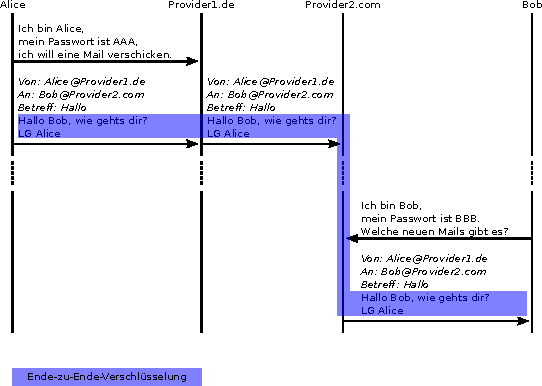
\includegraphics[width=.9\textwidth]{images/maildaten_e2e.pdf}
  \begin{itemize}
    \scriptsize
    \item unabhängig vom Mailanbieter möglich
    \item benötigt Zusatzsoftware und Schlüssel bei beiden Kommunikationspartnern
  \end{itemize}
\end{frame}

\begin{frame}{E-Mail}{Kombination Transport- und Ende-zu-Ende-Verschlüsselung}
  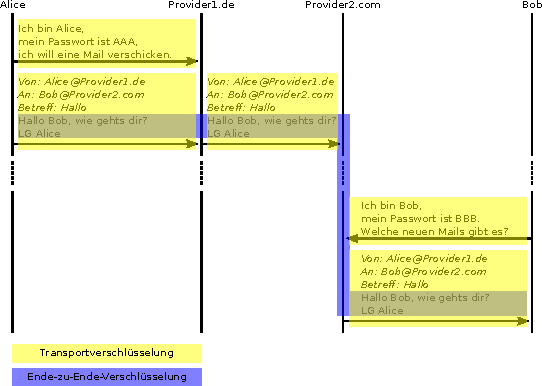
\includegraphics[width=.9\textwidth]{images/maildaten_beides.pdf}
  \scriptsize
  ~\\
  ~\\
\end{frame}

\begin{frame}{Authentizität öffentlicher Schlüssel}
Was, wenn A eine Nachricht an B schicken will,\\ aber den öffentlichen Schlüssel von B nicht kennt?\\
\begin{enumerate}
  \item Im ``Telefonbuch'' nach dem Schlüssel suchen
  \item Echtheit mit Hilfe eines \emph{vertrauenswürdigen Dritten} C überprüfen
\end{enumerate}
\begin{center}
  
\includegraphics[width=0.5\textheight]{images/vertrauen.pdf}
  %TODO: überarbeiten
\end{center}
\end{frame}

\begin{frame}{Wie stellt man Vertrauen in öffentliche Schlüssel her?}
  \begin{itemize}
    \item S/MIME -- Hierarchischer Vertrauensansatz
    \begin{itemize}
      \item hier nicht behandelt
    \end{itemize}
    \item OpenPGP -- Dezentraler Vertrauensansatz
    \begin{itemize}
      \item jeder kann festlegen, wem er vertraut
      \begin{itemize}
        \item er kann die Echtheit eines Schlüssels\\ z.B. bei einem persönlichen Treffen überprüfen
      \end{itemize}
      \item jeder \emph{kann} sein Vertrauensnetz veröffentlichen (Web-of-Trust)
      \begin{itemize}
        \item Vorteil: Man kann ``Freunden von Freunden'' vertrauen
        \item Nachteil: Beziehungen zwischen Menschen öffentlich\\ Aber: Facebook sagt da viel mehr aus
      \end{itemize}
      %\item wird hier behandelt
    \end{itemize}
  \end{itemize}
\end{frame}

\begin{frame}{Welche Software benötigt man?}
  \begin{block}{OpenPGP Backend}
    Macht die eigentliche Ver-/Entschlüsselung \& Signatur

    \vspace{1ex}
    \begin{tabular}{ccc}
      Linux:            & Windows: & Android:     \\
      \textit{on-board} & GPG4Win  & OpenKeychain \\
    \end{tabular}
  \end{block}
  \begin{block}{Plug-In fürs Mailprogram}
    Grafische Oberfläche, leichtere Schlüsselverwaltung, etc.

    \vspace{1ex}
    \begin{tabular}{ccc}
      Thunderbird: & Outlook: & K9-Mail: \\
      Enigmail     & GPG4Win  & --       \\
    \end{tabular}
  \end{block}
\end{frame}

\begin{frame}{Nächste Schritte:}
  \begin{enumerate}
    \item Software installieren (siehe vorige Folie)
    \item Installationsassistent starten
    \begin{enumerate}
      \item Schlüsselpaar erzeugen
      \item Passwort festlegen\\ (schützt privaten Schlüssel auf der Festplatte)
      \item Identitäten hinzufügen\\ (für welche E-Mail-Adresse(n) der Schlüssel gilt)
      \item Widerrufszertifikat auf USB-Stick speichern
      \item Öffentlichen Schlüssel auf Keyserver hochladen
    \end{enumerate}
    \item Erste verschlüsselte und signierte E-Mail schicken :)
  \end{enumerate}
\end{frame}

\endinput
